The tool spo2ida \citep{VamvatsikosCornell2005} is capable of converting static pushover curves into 16\%, 50\% and 84\% ida curves, as shown in Figure~\ref{fig:spo2ida}, using empirical relationships from a large database of incremental dynamic analysis results.

\begin{figure}[!htbp]
\centering
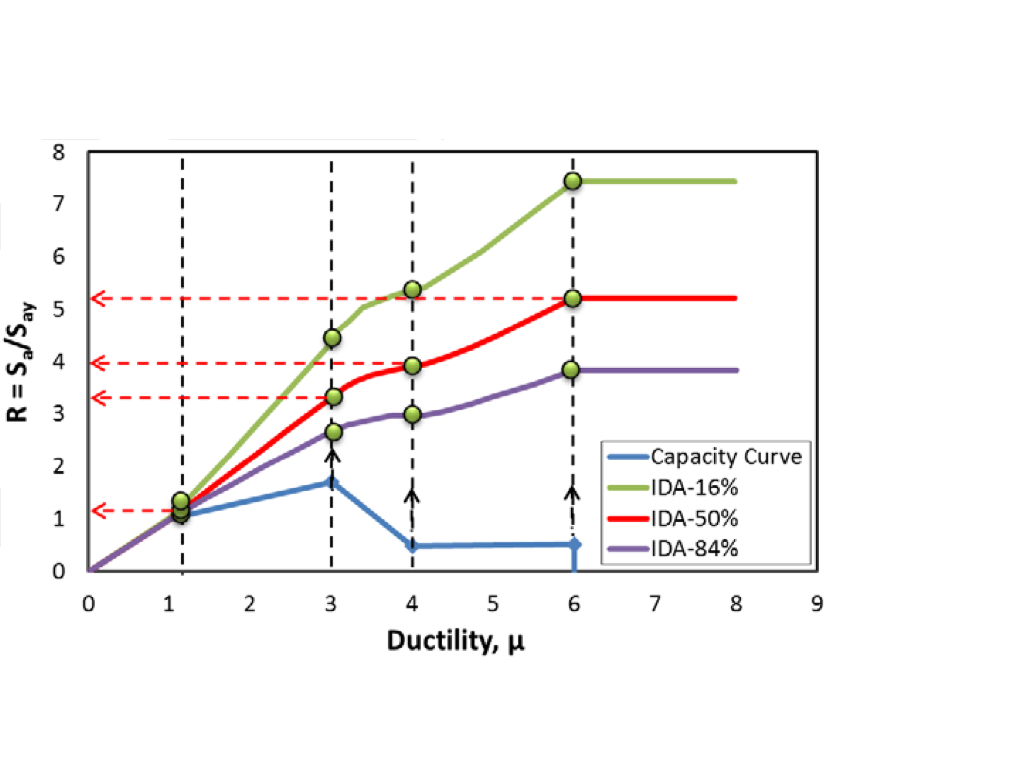
\includegraphics[width=10cm]{figures/spo2ida.jpg}
\caption{spo2ida tool: IDA curves derived from Pushover curve.}
\label{fig:spo2ida}
\end{figure}

The spo2ida tool is applicable to any kind of multi-linear capacity curve. Making use of this tool is is possible to estimate single building fragility curve and fragility curves derived for single buildings can be combined in a unique fragility curve, which considers also the inter-building uncertainty.\\

Given an idealised capacity curve the spo2ida tool uses an implicit R-$\mu$-T relation to correlate nonlinear displacement, expressed in terms of ductility $\mu$ to the corresponding median capacities in terms of the parameters R. R is the lateral strength ratio, defined as the ratio between the spectral acceleration S$_a$ and the yielding capacity of the system S$_{ay}$. Each branch of the capacity curve, hardening, softening and residual plateau, is converted to a corresponding branch of the three ida curves, using the R-$\mu$-T relation, which is a function of the hardening stiffness, the softening stiffness and the residual force. These parameters are derived from the idealised pushover capacity expressed in $\mu$-R terms, as well as the ductility levels at the onset of each branch. If some of the branches of the pushover curve are missing because of the seismic behaviour of the system, spo2ida can equally work with bilinear, trilinear and quadrilinear idealisations.\\

The result of the spo2ida routine is thus a list of ductility levels and corresponding R values at 50\%, 16\% and 84\% percentiles. For any inelastic displacement, and therefore any level of ductility $\mu$ the corresponding $R_{50\%}$, $R_{16\%}$, and $R_{84\%}$ values are found interpolating the aforementioned ida curves.
Median R and its dispersion at ductility levels corresponding to the damage thresholds ds can thus be determined, and converted into median $S_{a, ds}$ and its dispersion due to record-to-record variability $\beta_{S_{a d}}$ according to equations \ref{eq:SaR} and \ref{eq:betaR}. 

\begin{equation}
\hat{S}_{a, ds} = R_{50\%}(\mu_{ds}) S_{ay}
\label{eq:SaR}
\end{equation}
\begin{equation}
\beta_{S_{a d}} = \beta_{R(\mu_{ds})} = \frac{\ln R(\mu_{ds})_{84\%} - \ln R(\mu_{ds})_{16\%}}{2}
\label{eq:betaR}
\end{equation} 

If dispersion due to uncertainty in the limit state definition $\beta_{\theta c}$ is different from zero a Monte Carlo sampling needs to be performed to combine it with the record-to-record dispersion. Different values of ductility limit state are sampled from the  lognormal distribution with median the median value of the ductility limit state, and dispersion the input $\beta_{\theta c}$. For each of these ductilities the corresponding median $R_{50\%}$ and R$_{16\%}$, R$_{84\%}$ are found and converted into $\hat{S}_{a,ds}$ and $\beta_{S_{a d}}$ according to equation \ref{eq:SaR} and \ref{eq:betaR}. MC random S$_a$ for each MC sampled ductility limit state are computed, and their median and the dispersion are estimated. These parameters constitute the median $\hat{S}_{a,ds}$ and the total dispersion $\beta_{S_a}$ for the considered damage state. The procedure is repeated for each damage state.

\subsubsection{Multiple-Building Fragility and Vulnerability function}
\label{subsubsec:multiple-buildings}
If multiple buildings have been input to derive fragility function for a class of buildings all $\hat{S}_{a, blg}$ and $\beta_{S_a, blg}$ are combined in a single lognormal curve. A minimum of 5 buildings should be considered to obtain reliable results for the class.\\

A new issue arises when multiple buildings are considered: the S$_a$ at the fundamental period of each building should be converted to a common intensity measure, to be able to combine the different fragility functions. A common intensity measure is selected to be S$_a$ at the period T$_{av}$, which is a weighted average of the individual building fundamental periods T$_1$. Then each individual fragility needs to be expressed in terms of the common S$_a$(T$_{av}$), using a spectrum. FEMA P-695 \citep{ATC2007} far field set of 44 accelerograms (22 records for the two directions) was used to derive a mean uniform hazard spectrum, and the ratio between the S$_a$ at different periods is used to scale the fragility functions. It can be noted that the actual values of the spectrum are not important, but just the spectral shape. 
The median $\hat{S}_a$ is converted to the mean $\mu_{ln(S_a)}$ of the corresponding normal distribution ($\mu_{ln(S_a)} = ln(\hat{S}_a)$) and simply scaled to the common intensity measure as follows:

\begin{equation}
\mu_{ln(S_a), blg} = \mu_{ln(S_a), blg} S(T_{av})/ S(T_{1, blg})
\end{equation}
\begin{equation}
\beta_{S_a, blg} = \beta_{S_a, blg} S(T_{av})/ S(T_{1, blg})
\label{eq:Sa(Tav)}
\end{equation}

where $S(T_{av})/ S(T_{1, blg}$ is defined as spectral ratio. Finally the parameters of the single lognormal curve for the class of buildings, mean and dispersion, can be computed as the weighted mean of the single means and the weighted SRSS of the inter-building and intra-building standard deviation, the standard deviation of the single means and the single dispersions respectively, as shown in the following equations:

\begin{equation}
\mu_{ln(S_a), tot} = \sum_{i=0}^{n.blg} w_{blg-i} \mu_{ln(S_a), blg-i}
\label{eq:combination-lognormals-mu}
\end{equation}
\begin{equation}
\beta_{S_a, tot} = \sqrt{ \sum_{i=0}^{n.blg} w_{blg-i} ((\mu_{ln(S_a), blg-i}-\mu_{ln(S_a), tot})^2+ \beta_{S_a, blg-i}^2})
\label{eq:combination-lognormals-sigma}
\end{equation}

In order to use this methodology, it is necessary to load one or multiple capacity curves as described in Section \ref{subsec:cap_curves}. It is also necessary to specify the type of shape the capacity curves want to be idealised with, using the parameter \verb=idealised_type= (either \verb=bilinear= or \verb=quadrilinear=). If the user has already at disposal an idealised multilinear pushover curve for each building, the variable \verb=Idealised= in the csv input file should be set to \verb=TRUE=, and idealised curves should be provided according to what described in section \ref{subsec:cap_curves}. Then, it is necessary to specify a damage model using the parameter \verb=damage_model= (see Section \ref{subsec:dmg_model}).\\

If dispersion due to uncertainty in the limit state definition is different from zero a Monte Carlo sampling needs to be performed to combine it with the record-to-record dispersion. The number of Monte Carlo samples should be defined in the variable \verb=montecarlo_samples=.
After importing the module \verb=SPO2IDA_procedure=, it is possible to calculate the parameter of the fragility model, median and dispersion, using the following command:

\begin{Verbatim}[frame=single, commandchars=\\\{\}, samepage=true]
fragility_model = SPO2IDA_procedure.calculate_fragility(capacity_curves,
... idealised_capacity, damage_model, montecarlo_samples, Sa_ratios,
... ida_plotflag)
\end{Verbatim}

where \verb=Sa_ratios= is the spectral ratio variable needed to combine together fragility curves for many buildings, as described in Section \ref{subsec:derive_fragility}, and \verb=ida_plotflag= indicates whether ida plots want to be displayed (\verb=ida_plotflag= = 1) or not (\verb=ida_plotflag= = 0).